\documentclass{article}

\usepackage[nodayofweek,level]{datetime}
\usepackage[autostyle, english = american]{csquotes}
\usepackage{graphicx}
\usepackage{multicol}
\usepackage[margin=0.5in]{geometry}
\MakeOuterQuote{"}

\begin{document}

\title{Assemble: An Audio-Spatial Deliberation Platform}
\date{October 13, 2016}
\author{A Thesis Proposal, by Ben Packer}

\maketitle{}

\section{Introduction}

As information technologies developed and new communication technologies that
compressed the space and latency between participants gained popularity, many
optimistic theorists of collective decision-making predicted a democratic
revolution throughout governments, civil organizations, and businesses, flattening
heirarchies and correcting information imbalances \cite{hartz}.

\medskip

Unfortunately, although the exact effect of new communication technologies on
decision-making practices is unclear, it is clear that the participatory revolution
did not happen as foreseen \cite{hartz}.

\medskip

Although there are many cultural and institutional barriers to the adoption of
new methods of decision-making, it is at least partly a problem of design \cite{towne}. Computer
platforms used for participatory communication have a unique set of design challenges,
including accomodating the flexibility of offline decision-making \cite{seeds},
maintaining coherence, order, and direction as the number of participants increases \cite{pingree},
creating an equitable, coercion-free discourse environment that facillitates inclusive
discussion \cite{habermas}, and making computer-mediated meetings efficient, fun, and satisfying
enough that people choose participatory decision-making over acquiesence to
hierarchy \cite{graeber}\cite{lupia}.

\section{Existing Platforms and My Solution}

The current landscape of platforms to facillitate participatory deliberation online has
saturated its small user base. There are many platforms
(Loomio \cite{loomio}, DemocracyOS \cite{dos}, Hylo \cite{hylo}, and Liquid Feedback \cite{lf}),
but none have yet to challenge the primary of simple forums, email chains,
chatrooms, group video chats, conference calls, and other general-purpose
computer mediated communication technologies \cite{}.

\medskip

Although any explanation for why groups that want to make decisions democratically prefer
general purpose communication tools over dedicated solutions remains untested, my intuition
is that each tool forces the group to make decisions a particular way. In other words,
the features these platforms provide are too "opinionated", with each additional feature
requiring additional adaptation in the group's methods. Owing to
the importance that these groups place on their methods of decision-making, it is
not surprising that they choose general purpose, flexible tools over dedicated platforms
and custom workarounds over constraints.

\medskip

Thus, I propose a design for a collective decision making platform based on a few,
simple, \textit{rules} governing interaction in an open environment instead of a
feature-per-necessity designed platform. My hope is that such a platform will be
flexible enough for users to easily transfer their existing decision processes
but principled enough that the platform encourages participation by the nature of its
design.

\section{Assemble}

My solution, which I am currently calling \textit{Assemble}, is to re-create
two, obvious, environmental rules that enable widespread flexibility in offline decision-making.
First, people can talk to each other. Second, as \textit{A} moves further away from
\textit{B}, \textit{A} and \textit{B} can hear each other less well. The first is an
ability, and the second is a constraint on that ability. To understand the importance
of the constraint, imagine trying to break into subgroups on a conference call,
or how impossible it would be to have a conversation if everyone in the world could
hear everyone else equally well.

\medskip

Using browser based technologies to ensure the lowest barrier to participation, I have
built a prototype of the above implementing just those two features, using ReactJS,
Socket.io, and WebRTC.


\begin{figure}[ht!]
\centering
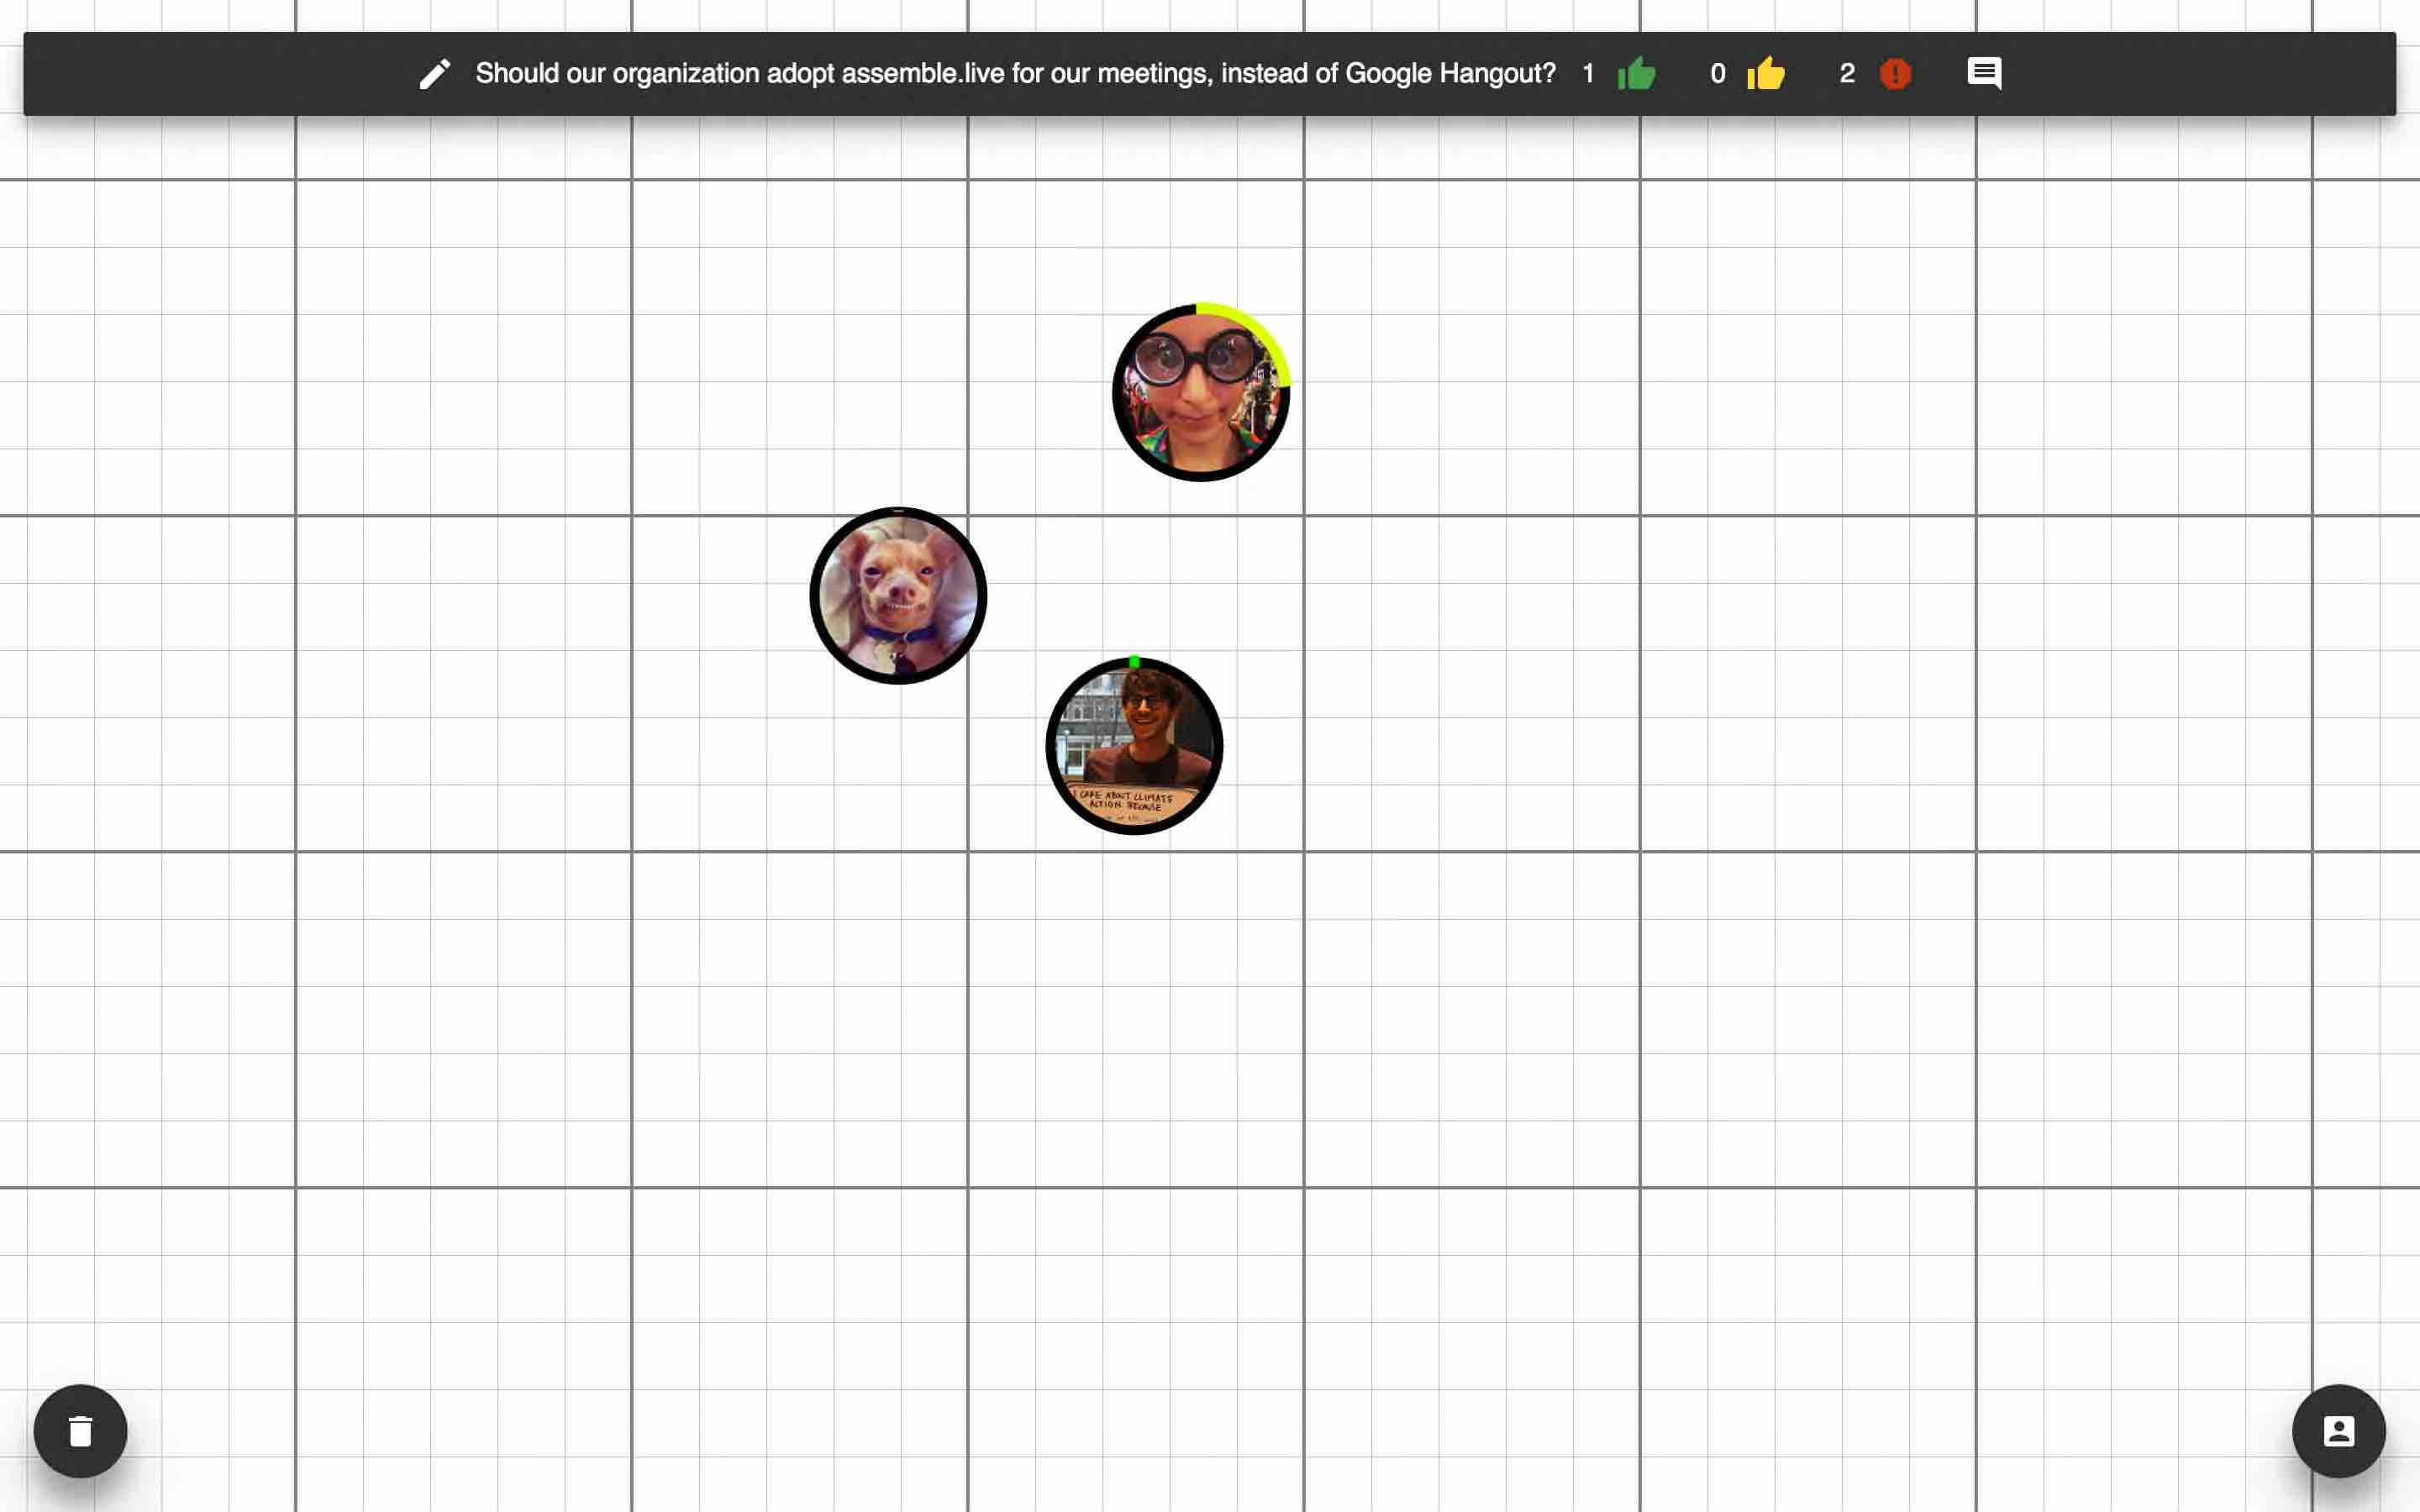
\includegraphics[width=90mm]{./papers/proposal/screenshot.jpg}
\caption{Screenshot of use on August 14, 2016.}
\end{figure}


Movement is accomplished by clicking and holding where you want to go, and as you move further
away from the other participants, the volume at which you hear them decreases. I have
managed to test this prototype with as many as 12 moving and talking participants with
no noticable increase in latency or trouble transferring audio.

\section{Challenges and Plans}

\textit{Assemble} is far from being a usable and effective way to make
decisions online. The following are a minimal list of what is needed before
the platform offers benefits over a multi-party video chat with a collaborative
document.

\begin{enumerate}
  \item Testing and Optimization \\
  Being a real-time platform that only derives its market advantage in larger groups (7+),
  it is important that the platform be heavily optimized and tested to run laglessly
  and buglessly with a large number of participants.
  \item Note Taking and Permanence \\
  \textit{Assemble} does not at the moment support any method of note-taking, a practice essential
  to modern meetings that need to be referenced in the future or where not all relevant
  stakeholders are in attendence. Options for filling this gap include live document
  co-editing and chat features.
  \item Security Assurances \\
  Since many meetings discuss sensitive information, \textit{Assemble} will need
  to be fully secure and private, requiring a migration from its current, all public
  room model to the creation of private rooms with end-to-end encrypted text communication.
  \item Accessibility \\
  Since it is based on an audio/visual environment, \textit{Assemble} raises special
  accessibility concerns for low-hearing and low-vision users. Such concerns are magnified
  in deliberation, where the exclusion of a handicapped group may have profound exclusionary
  effects on policy reached. Thus, I aim to make \textit{Assemble} fully usable through
  only one sense (audio-only / visual-only, accomplished through voice commands and
  speech-to-text conversation).
\end{enumerate}

\section{Timeline}

\textit{Dates are estimates}

\textbf{November 30 - January 4} \\
Stabilize, optimize, and secure current feature set, including the core audio-spatial
engine, agenda setting and voting features, and post-meeting digests, in preparation for
the first round of user testing.

\textbf{January 5 - January 20} \\
User testing with Dartmouth students and online communities I am a member of.

\textbf{January 20 - March 24} \\
Implement improvements suggested by user testing, move towards live document co-editing
and/or chat, and improve the accessibility of the platform.

\textbf{March 26 - April 10} \\
Another round of user testing

\textbf{April 10 - May 1} \\
Implement improvements suggested by user testing, rounding out the feature set for
a beta launch.

\textbf{May 1 - May 30} \\
Write up of thesis project, including attempts at attracting the attention
of the open source development community and the academic online deliberation field.

\section{Advisors}
Seth Frey and Tim Tregubov.

\begin{thebibliography}{9}

\bibitem{pingree}
Pingree, R. J. (2009). Decision structure: A new approach to three problems in deliberation. \textit{Online deliberations: design, research, and practice. CSLI Publications, San Francisco, CA}, 309-316.

\bibitem{towne}
Towne, W. B., \& Herbsleb, J. D. (2012). Design considerations for online deliberation systems. \textit{Journal of Information Technology \& Politics}, 9(1), 97-115.

\bibitem{habermas}
Habermas, J. (1991). \textit{The structural transformation of the public sphere: An inquiry into a category of bourgeois society}. MIT press.

\bibitem{graeber}
Graeber, D. (2013). \textit{The democracy project: A history, a crisis, a movement}. Spiegel \& Grau.

\bibitem{lupia}
Lupia, A. (2009). Can online deliberation improve politics? \textit{Scientific foundations for success. Scientific Foundations for Success.}

\bibitem{seeds}
Ltd, Seeds For Change Lancaster Co-Operative. (2013). \textit{Consensus handbook: Co-operative decision making for activists, co-ops and communities.}

\bibitem{hartz}
Hartz-Karp, J., \& Sullivan, B. (2014). \textit{The unfulfilled promise of online deliberation. Journal of Public Deliberation}, 10(1).

\bibitem{loomio}
(n.d.). Loomio | Make Decisions Together. Retrieved October 13, 2016, from https://www.loomio.org/

\bibitem{dos}
DemocracyOS. (n.d.). Retrieved October 13, 2016, from http://democracyos.org/

\bibitem{lf}
LiquidFeedback. (n.d.). Retrieved October 13, 2016, from http://liquidfeedback.org/

\bibitem{hylo}
Hylo. (n.d.). Retrieved October 13, 2016, from https://www.hylo.com/


\end{thebibliography}


\end{document}
